\subsection{Realizing LBM Models with DEM Packing}
In \cref{sec:lbm-equations} we introduced the basic mechanics and governing equations behind mass, momentum, and energy transport with the lattice-Boltzmann method. Because of the immensely simple implementation of no-slip boundary conditions for even the most complex geometry, the lattice-Boltzmann method was immediately seen as a powerful option of fluid modeling in porous networks after its introduction. Chen \& Doolen review many of the major accomplishments of implementing LBM models which verified Darcy's Law, the Cozeny-Karman equation, and Brinkmann equation among other efforts.\cite{Chen1998a} Pan\etal~evaluated the single-relaxation time BGK operator against models with multiple relaxation times as well as the differences with implemented various fluid-solid interface boundary conditions -- among which was the bounce-back scheme we use here.\cite{Pan2006}

Here we will go through the practical application of the LBM approach as we use it to simulate the conjugate heat transfer of the helium purge gas through our packed bed. To summarize the method, there are two main objects required to define the structure of a lattice-Boltzmann model: a collision operator, $\Omega_i$, and the constants which define the scaffolding of the lattice, $q$, $\vec{c}_i$, $c_s$, and $w_i$.

\begin{figure}[ht]
	\centering
	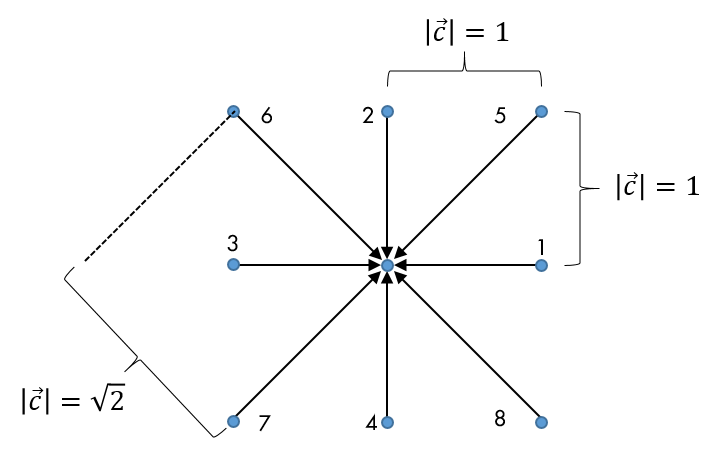
\includegraphics[width=\singleimagewidth]{chapters/figures/lbm/d2q9-lattice.png}
	\caption{A representative node with directional vectors to the 8 neighbors (+1 central node) in the D2Q9 lattice.}\label{fig:d2q9-lattice}
\end{figure}

The computational domain of the fluid is discretized into a Cartesian grid with regularized spacing, $\delta_x$, in every dimension. At each node are density functions, $f_i(\vec{x},t)$, which represent the density at that node (found at $\vec{x}$), traveling in the direction of $\vec{c}_i$ at a moment in time, $t$. We will be solving the equations through a three-dimensional pebble bed, but use a common two-dimensional lattice for demonstration purposes. Given in Fig.~\ref{fig:d2q9-lattice} is a node in a D2Q9 lattice; the directions and lengths of the velocity vectors are shown.

The density distribution function evolves according to Eq.~\ref{eq:lbm-evolution}. It is given again here for reference,
\begin{align}
	\underbrace{f_i(\vec{x}+\vec{c}_i, t + 1)  = f_i(\vec{x},t)}_\text{streaming}  + \underbrace{\Omega_i(\vec{x},t)}_\text{collision}
\end{align}

Conceptually the evolution can be thought of as two distinct operations. First, the collision operator is calculated based only on each nodes local information. Using the BGK approximation, given in Eq.~\ref{eq:bgk-operator}, the collision is calculated as
\begin{align}
	\Omega_i = -\frac{1}{\tau}\left[f_i(\vec{x},t) - f_i^\eq(\vec{x},t)\right]
\end{align}

Post-collision, in the streaming step, the information is passed from the node to its neighbors along the lattice directions shown in Fig.~\ref{fig:d2q9-lattice}. While the collision operation is exactly local, the streaming operation involves only nearest neighbors. After the streaming step, the nodes that lie along the boundary have some particle distributions that are unknown as their neighbors lie outside the domain. In these cases, the bounce-back boundary condition is applied wherein distributions arriving at the boundary are reflected back to their incident directions. The bounce-back calculation enforces no-slip at the walls.

Splitting the evolution of the distribution function into the two steps of collision and streaming, in addition to being a conceptual aid, is a natural partition of computational steps. In practice the algorithm proceeds as follows,\cite{Viggen2009}
\begin{enumerate}
	\item{using macroscopic properties of density and fluid velocity, the equilibrium distribution function is calculated at every node following Eq.~\ref{eq:equilib-dist-function}}
	\item{the BGK collision operator is calculated according to Eq.~\ref{eq:bgk-operator} to find the post-collision distribution of every node}
	\item{information from each node is propagated to neighboring nodes based on the evolution equation of Eq.~\ref{eq:lbm-evolution}.}
	\item{updated macroscopic properties are found from the new distribution functions according to Eq.~\ref{eq:lbm2physical}.}
\end{enumerate}

It is worth stressing again that the lattice-Boltzmann calculations are completely local, with the streaming step requiring only inter-node communication for updating distribution functions. With the approach clearly laid out, we now need only incorporate our pebble bed into the LBM computational space.



\subsection{Mapping DEM Pebbles onto LBM Nodes}

Unlike the direct coupling between DEM and the volume-averaged CFD, we are limited here to translating a static packing structure from DEM into the LBM framework. The lattices of the LBGK solver use equally spaced nodes that discretize our volume at normal intervals. The pebble data from DEM is mapped onto the LBM nodes via knowledge of the centroid and radius of each pebble. To demonstrate, in Fig.~\ref{fig:dem-2-lbm-example1}, we see a two-dimensional slice of a pebble projected onto a section of an LBM lattice. If the distance from a node to the centroid is less than the radius of the pebble, the node is assigned as a solid. All other nodes are assigned as fluids.

\begin{figure}[ht]
	\centering
	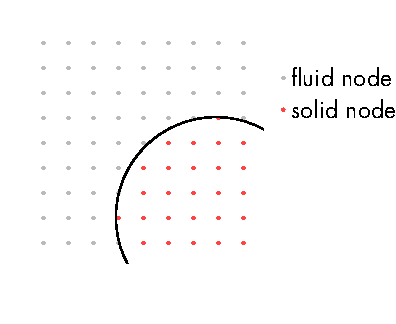
\includegraphics[width=\singleimagewidth]{chapters/figures/lbm/dem-to-lbm-mapping.pdf}
	\caption{An example of the mapping process from DEM to LBM structures. Nodes are assigned as fluid or solid based on relative location of pebble centroid and radius. Here we have a resolution of 9 (\textit{i.e.} 9 nodes per pebble diameter).}\label{fig:dem-2-lbm-example1}
\end{figure}
\begin{figure}[ht]
	\centering
	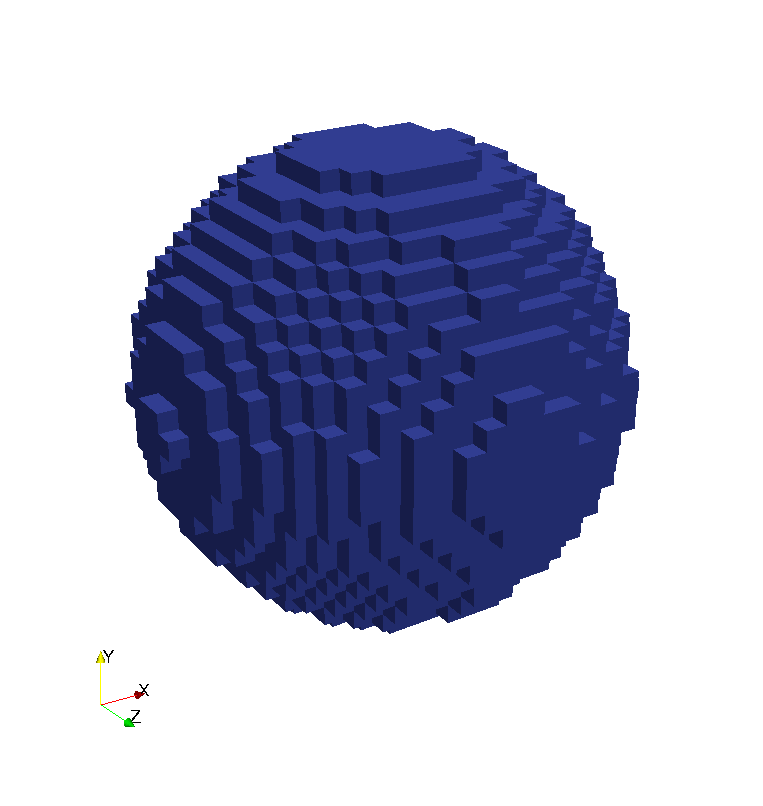
\includegraphics[width=\doubleimagewidth]{chapters/figures/lbm/lbm-pebble-res25.png}
	\caption{A three-dimensional DEM pebble as imported into the LBM lattice with a resolution of 25.}\label{fig:dem-2-lbm-example2}
\end{figure}
\begin{figure}[ht]
	\centering
	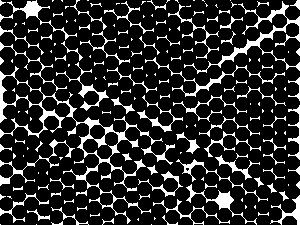
\includegraphics[width=\doubleimagewidth]{chapters/figures/lbm/crossSection0024.jpg}
	\caption{A two-dimensional slice of a DEM pebble bed as imported into the LBM lattice with a resolution of 25.}\label{fig:dem-2-lbm-example3}
\end{figure}
\begin{figure}[ht]
	\centering
	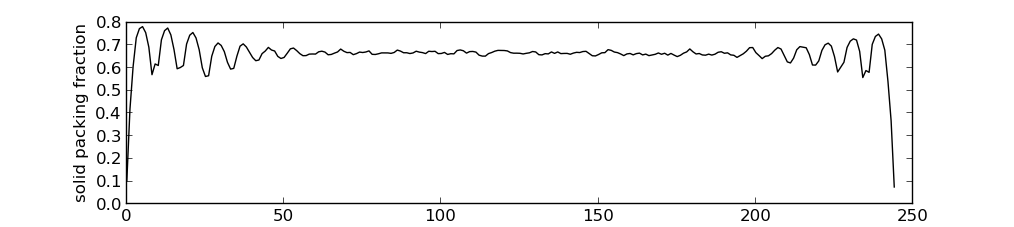
\includegraphics[width=\textwidth]{chapters/figures/lbm/palabos_packing_fraction}
	\caption{The digital packing fraction was measured at all slices through the height of the pebble bed. When the average value equaled the expected value, the mapping from DEM to LBM was considered consistent.}\label{fig:dem-2-lbm-packing-fraction}
\end{figure}

In the example of Fig.~\ref{fig:dem-2-lbm-example1}, the resolution is only 9. Thus 9 nodes are needed to span the diameter of a single pebble and the lattice spacing is $\delta_x = 1/9$. In the second example shown in Fig.~\ref{fig:dem-2-lbm-example2}, we see a pebble in three dimensions that has been mapped onto the LBM nodes with a resolution of 25 (thus $\delta_x = 1/25$). The trade-off between a small lattice spacing is in the ability to resolve the spherical surface of the pebble, stability, and even the ability to resolve a proper packing fraction in the pebble bed. 

Shown in Fig.~\ref{fig:dem-2-lbm-example3} is a single slice of a pebble bed with a resolution of 25 as it is mapped into LBM. Here, black pixels represent solid and white pixels are fluid. Because we are representing the surfaces of curved objects with straight lines, at the point of contact between pebbles, the mapping from DEM to LBM would occasionally over-predict the overlap between pebbles. This was measured numerically by comparing the number of white pixels to black pixels in each slice -- the digital equivalent of a packing fraction,
\begin{equation}
	\phi_{d,j} = \frac{N_\text{black}}{N_\text{white}}
\end{equation}

The total digital packing fraction of the ensemble, as mapped into LBM, is simply
\begin{equation}
	\phi_d = \frac{1}{J}\sum_j^J\phi_{d,j}
\end{equation}

where there are $J$ total slices. For example, we see in Fig.~\ref{fig:dem-2-lbm-packing-fraction} a plot of the digital packing fraction moving through a pebble bed we had analyzed. The digital mapping of DEM onto LBM was tweaked with a radius magnification parameter until the digital packing fraction matched the calculated packing fraction from DEM. When the error between digital and continuous packing fractions was small, as calculated by
\begin{equation}
	\Phi_{err} = \frac{|\phi_d - \phi|}{\phi} < 10^{-4}
\end{equation}

we considered the mapping from DEM to LBM to be consistent.
\FloatBarrier